\documentclass{article}
\usepackage{amsmath}
\usepackage{graphicx} % Required for inserting images
\usepackage{float} % For figures placement
\usepackage{fancyvrb} % for \Verb
\usepackage[a4paper, margin=2.5cm]{geometry}
\usepackage{karnaugh-map} % Tableau de Karnaugh
% Subfigures
\usepackage{caption}
\usepackage{subcaption}
\usepackage{multicol}

\usepackage{amsmath}
\usepackage{emoji}

\usepackage{enumitem}

\usepackage{tikz}
\usetikzlibrary{automata, positioning, arrows}

\usepackage[hidelinks]{hyperref}


\usepackage{listings}
\usepackage{xcolor}

\definecolor{codegreen}{rgb}{0,0.6,0}
\definecolor{codegray}{rgb}{0.5,0.5,0.5}
\definecolor{codepurple}{rgb}{0.58,0,0.82}
\definecolor{backcolour}{rgb}{0.95,0.95,0.92}

\lstdefinestyle{mystyle}{
    backgroundcolor=\color{backcolour},   
    commentstyle=\color{codegreen},
    keywordstyle=\color{magenta},
    numberstyle=\tiny\color{codegray},
    stringstyle=\color{codepurple},
    basicstyle=\ttfamily\footnotesize\linespread{0.1},
    breakatwhitespace=false,         
    breaklines=true,                 
    captionpos=b,                    
    keepspaces=true,                 
    numbers=left,                    
    numbersep=5pt,                  
    showspaces=false,                
    showstringspaces=false,
    showtabs=false,                  
    tabsize=2,
}

\newcommand{\lstbg}[3][0pt]{{\fboxsep#1\colorbox{#2}{\strut #3}}}
% \lstdefinelanguage{diff}{
%   basicstyle=mystyle,
%   morecomment=[f][\lstbg{red!20}]-,
%   morecomment=[f][\lstbg{green!20}]+,
%   morecomment=[f][\textit]{@@},
%   %morecomment=[f][\textit]{---},
%   %morecomment=[f][\textit]{+++},
% }

\lstset{
    language=C++,
    style=mystyle,
}

\usepackage{setspace} % to change line spacing
\renewcommand{\baselinestretch}{1.5} 


\setlength{\parskip}{\baselineskip}%
\setlength{\parindent}{0pt}%

\begin{document}

\makeatletter
\begin{titlepage}
\begin{center}
    

\includegraphics[width=7cm]{assets/LogoCN_Q.png}
\\
\textbf{\large{Centrale Nantes}}
\\[2cm]

\textbf{\large{MAC : $6^{th}$ Lab's Report \\
Interrupts --- Ultrasonic sensor }}
\\[14pt]
$1^{st}$ year Embedded Systems Engineering
\\[2cm]


\vfill

\textbf{By} \\
EL KHAYDER Zakaria \\
SAOUTI Rayan
\\[1cm]

\textbf{Professor} \\
BRIDAY Mikael
\\[3cm]

February 09, 2023 \\ [12pt]

Session \\
2023-2024 \\[12pt]
\small{Made with \LaTeX}
\end{center}
\end{titlepage}
\makeatother

\pagebreak

\setcounter{page}{1}
\pagenumbering{Roman}

\clearpage
\addcontentsline{toc}{section}{Contents}
\tableofcontents

\clearpage
\addcontentsline{toc}{section}{Listings}
\lstlistoflistings

\clearpage

\setcounter{page}{1}
\pagenumbering{arabic}

\section{Encoder}

Unlike the actual process we followed in this lab, we will start this report by implementing the \verb|Rotating encoder| code given it is relatively the simplest in this project.

\subsection{Logic}

We should implement an external interrupt (falling edge) on one of the two encoder inputs, and read the state of the other one. With these two states, we can determine the rotation direction based on the following figure.

\begin{figure}[H]
    \centering
    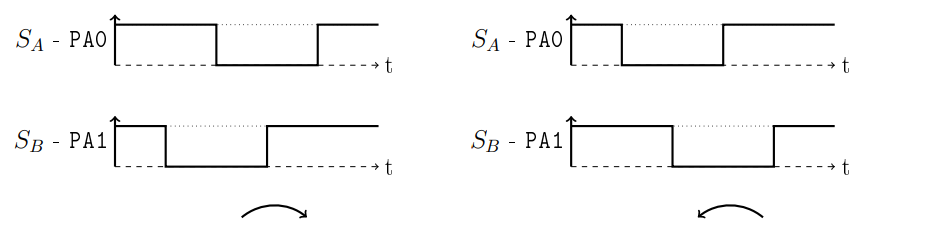
\includegraphics[width=12cm]{assets/encoder_logic.png}
\end{figure}

\subsection{Implementation}

\subsubsection{Setup}

We chose to link the external interrupt on $S_A$ (PA0). Luckily this is easy thanks to the already provided \verb|pinMode| and \verb|attachInterrupt|.

This logic will be available in the \verb|encoderInit| function to simplify the API usage for the user.

\begin{lstlisting}[language=C++, caption={encoderInit Implementation}]
void encoderInit(void)
{
    pinMode(GPIOA, 0, INPUT_PULLUP);
    pinMode(GPIOA, 1, INPUT_PULLUP);

    attachInterrupt(GPIOA, 0, FALLING);
}
\end{lstlisting}

\subsubsection{Interrupt handler}

The interrupt is linked to \verb|EXTI0|. \\
Once the interrupt is triggered, we should read the state of the other pin ($S_B$), and based on its state, we can deduct the rotation direction.

\begin{lstlisting}[language=C++, caption={EXTI0\_IRQHandler Implementation}]
extern "C" void EXTI0_IRQHandler(void)
{
    if (digitalRead(GPIOA, 1) == 0) { // SA == 0 & SB == 0 => Clockwise => Increment
        if (_encoderValue < 45) // < Max
            _encoderValue++; 
    } else { // SA == 0 & SB == 1 => Counter Clockwise => Decrement
        if (_encoderValue > 0) // > Min
            _encoderValue--; 
    }
    EXTI->PR |= EXTI_PR_PR0; // acknowledge
}
\end{lstlisting}

\subsubsection{State}

The \verb|__encoderValue| is a private (local) integer variable in the current file (encoder.cpp). We can get the value of the said variable using a simple getter function.

\begin{lstlisting}[language=C++, caption={\_encoderValue getter}]
int encoderValue(void) { return _encoderValue; }
\end{lstlisting}


We are doing things this way to forbid (or at least discourage) the user from changing the value of the \verb|_encoderValue| variable directly.

\section{ServoMotor}

The \verb|ServoMotor| rotation degree depends on the input PWM signal ON time (f = 50Hz). The output rotation degree goes linearly from 0deg at PWM$_{on}$ = 1ms to 90deg at PWM$_{on}$ = 2ms.

\subsection{Init}

PWM signal generation is kin of complicated to config on STM32, but it can be divided into 3 steps:

\begin{itemize}
    \item Output pin config with alt mode
    \item Timer config
    \item Pin/Timer and channel linking
\end{itemize}

\begin{lstlisting}[language=C++, caption={servoInit}]
#define PB0 GPIOB, 0

void servoInit()
{
    // 1. Output config
    pinMode(PB0, OUTPUT);
    pinAlt(PB0, 2);

    // Input clock = 64MHz.
    RCC->APB1ENR |= RCC_APB1ENR_TIM3EN;
    // Reset peripheral (mandatory!)
    RCC->APB1RSTR |= RCC_APB1RSTR_TIM3RST;
    RCC->APB1RSTR &= ~RCC_APB1RSTR_TIM3RST;

    // 2. Configure timer
    TIM3->CNT = 0;         // Reset
    TIM3->SR = 0;          // Reset
    TIM3->PSC = 64 - 1;    // 1MHz
    TIM3->ARR = 20000 - 1; // 20ms

    // 3. PWM configuration
    TIM3->CCMR2 &= ~TIM_CCMR2_CC3S_Msk;     // channel 3 as output
    TIM3->CCMR2 |= 6 << TIM_CCMR2_OC3M_Pos; // output PWM mode 1
    TIM3->CCMR2 |= TIM_CCMR2_OC3PE;         // Pre-load register TIM3_CCR3
    TIM3->CR1 &= ~TIM_CR1_CMS_Msk;          // mode 1 // edge-aligned mode
    TIM3->CR1 |= TIM_CR1_CEN;               // enable
    TIM3->CCER |= TIM_CCER_CC3E;            // enable
    TIM3->CCR3 = 1000 - 1;                  // Start at 1ms (0 deg)
}
\end{lstlisting}

\subsection{Rotate}

\begin{lstlisting}[language=C++, caption={servoSet}]
void servoSet(int setPoint)
{
    if (setPoint < 0) // MIN
        setPoint = 0;
    else if (setPoint > 1000) // MAX
        setPoint = 1000;

    TIM3->CCR3 = 1000 + setPoint - 1;
}
\end{lstlisting}

The \verb|servoSet| function takes a value between 0 and 1000, but our \verb|Rotary Encoder| API returns a value between 0 and 90 instead, we can add a helper function to do the translation between the two parts (declared in encoder.cpp)

\begin{lstlisting}[language=C++, caption={encoderValueInSteps}]
int encoderValueInSteps(void)
{
    return (_encoderValue * 1000) / 90;
}
\end{lstlisting}

\section{Application}

Now that we have implemented the cores of our project, we can move into actually using them to build something of value.

\subsection{Manual Mode}

The manual mode is straightforward, we should just copy the value of the \verb|Rotary Encoder| to the PWM output, and thanks to our already implemented function, it is as easy as the following line

\begin{lstlisting}[language=C++, caption={Manual Mode one-liner}]
    	servoSet(encoderValueInSteps());
\end{lstlisting}

\subsection{Scan Mode}

For the scan mode, we have to add a variable to keep track of our current rotation angle (we used a steps tracker instead for higher precision).
We will also need a function to be called periodically (using a timer interrupt) to increase or decrease the current rotation angle (Value between 0deg and 45deg).

\subsubsection{Timer}
We decided to go with \verb|TIM6|, with a period of 100ms (rotation speed was chosen pseudo-randomly).

\begin{lstlisting}[language=C++, caption={TIM6 Config}]
    // input clock = 64MHz.
    RCC->APB1ENR |= RCC_APB1ENR_TIM6EN;
    // reset peripheral (mandatory!)
    RCC->APB1RSTR |= RCC_APB1RSTR_TIM6RST;
    RCC->APB1RSTR &= ~RCC_APB1RSTR_TIM6RST;

    // Configure timer
    TIM6->CNT = 0;
    TIM6->SR = 0;
    TIM6->PSC = 64000 - 1; // 1ms
    TIM6->ARR = 10 - 1;    // 100ms
    TIM6->CR1 = 1;

    // Enable interrupt
    TIM6->DIER |= TIM_DIER_UIE;
    NVIC_EnableIRQ(TIM6_DAC1_IRQn);
\end{lstlisting}

\subsubsection{Handler}

\begin{lstlisting}[language=C++, caption={Scan Mode handler}]
    // Verify bounds
    if (_steps <= 0)
        _dir = Direction::Clockwise;
    else if (_steps >= 500)
        _dir = Direction::CounterClockwise;
        
    // Rotate
    if (_dir == Direction::Clockwise)
        _steps++;
    else // CounterClockwise
        _steps--;
\end{lstlisting}

\subsection{Transition mode}

To switch between the two previous modes (Scan and Manual) we will need an extra mode adequately named \verb|Transition Mode|.

If we switch directly from \verb|Scan| to \verb|Manual|, and the current \verb|Rotary Encoder| value is different from the \verb|Scan Mode| steps, the motor will suddenly jump from one position to another in a blink, which may damage the motor.

To avoid this, the \verb|Transition Mode| will act as an intermediate step between the two modes, only in one way (Scan to Manual) as the other way around is safe to switch directly.

\begin{figure}[H]
    \centering
    \tikzset{every picture/.style={line width=0.75pt}} %set default line width to 0.75pt        
    \begin{tikzpicture}[x=0.75pt,y=0.75pt,yscale=-1,xscale=1]
        %uncomment if require: \path (0,365); %set diagram left start at 0, and has height of 365
        %Flowchart: Connector [id:dp3458507959598227] 
        \draw   (272.49,82.12) .. controls (272.49,54.44) and (295.55,32) .. (323.99,32) .. controls (352.43,32) and (375.49,54.44) .. (375.49,82.12) .. controls (375.49,109.81) and (352.43,132.25) .. (323.99,132.25) .. controls (295.55,132.25) and (272.49,109.81) .. (272.49,82.12) -- cycle ;
        %Curve Lines [id:da708744711664278] 
        \draw    (272.49,82.12) .. controls (189.04,93.52) and (92.48,181.49) .. (159.64,262.78) ;
        \draw [shift={(160.66,264.01)}, rotate = 229.73] [color={rgb, 255:red, 0; green, 0; blue, 0 }  ][line width=0.75]    (10.93,-3.29) .. controls (6.95,-1.4) and (3.31,-0.3) .. (0,0) .. controls (3.31,0.3) and (6.95,1.4) .. (10.93,3.29)   ;
        %Flowchart: Connector [id:dp9563768804336197] 
        \draw   (160.66,264.01) .. controls (160.66,229.99) and (188.99,202.42) .. (223.93,202.42) .. controls (258.88,202.42) and (287.2,229.99) .. (287.2,264.01) .. controls (287.2,298.02) and (258.88,325.59) .. (223.93,325.59) .. controls (188.99,325.59) and (160.66,298.02) .. (160.66,264.01) -- cycle ;
        %Flowchart: Connector [id:dp13423656165195186] 
        \draw   (390.2,238.23) .. controls (390.2,210.54) and (413.26,188.1) .. (441.7,188.1) .. controls (470.14,188.1) and (493.2,210.54) .. (493.2,238.23) .. controls (493.2,265.91) and (470.14,288.35) .. (441.7,288.35) .. controls (413.26,288.35) and (390.2,265.91) .. (390.2,238.23) -- cycle ;
        %Curve Lines [id:da6392713290566039] 
        \draw    (287.2,264.01) .. controls (345.76,221.26) and (362.08,327.38) .. (420.22,286.12) ;
        \draw [shift={(421.1,285.49)}, rotate = 143.87] [color={rgb, 255:red, 0; green, 0; blue, 0 }  ][line width=0.75]    (10.93,-3.29) .. controls (6.95,-1.4) and (3.31,-0.3) .. (0,0) .. controls (3.31,0.3) and (6.95,1.4) .. (10.93,3.29)   ;
        %Curve Lines [id:da2219811564761307] 
        \draw    (479.95,200.99) .. controls (538.51,158.24) and (500.93,78.63) .. (377.35,82.07) ;
        \draw [shift={(375.49,82.12)}, rotate = 358.03] [color={rgb, 255:red, 0; green, 0; blue, 0 }  ][line width=0.75]    (10.93,-3.29) .. controls (6.95,-1.4) and (3.31,-0.3) .. (0,0) .. controls (3.31,0.3) and (6.95,1.4) .. (10.93,3.29)   ;
        % Text Node
        \draw (305.99,71.48) node [anchor=north west][inner sep=0.75pt]   [align=left] {Scan};
        % Text Node
        \draw (416.93,229.01) node [anchor=north west][inner sep=0.75pt]   [align=left] {Manual};
        % Text Node
        \draw (117.63,157.73) node [anchor=north west][inner sep=0.75pt]  [font=\small,rotate=-305.36] [align=left] {Button click};
        % Text Node
        \draw (326.1,276.4) node [anchor=north west][inner sep=0.75pt]  [font=\small,rotate=-29.14] [align=left] {\_steps = \_pos};
        % Text Node
        \draw (458.24,104.23) node [anchor=north west][inner sep=0.75pt]  [font=\small,rotate=-61.03] [align=left] {Button click};
        % Text Node
        \draw (191.17,259.09) node [anchor=north west][inner sep=0.75pt]   [align=left] {Transition};
    \end{tikzpicture}
    \caption{Modes switching}
\end{figure}

\begin{lstlisting}[language=C++, caption={Mode Switching handler}]
extern "C" void EXTI1_IRQHandler(void)
{
    switch (_mode)
    {
    case Mode::Scan:
    case Mode::Transition:
        _mode = Mode::Transition;
        break;

    case Mode::Manual:
        _steps = encoderValueInSteps();
        _mode = Mode::Scan;
        break;
    }
    EXTI->PR |= EXTI_PR_PR1; // acknowledge
}

\end{lstlisting}

\begin{lstlisting}[language=C++, caption={Updated Rotation TIM6 handler}]
extern "C" void TIM6_DAC1_IRQHandler(void)
{
    if (_mode == Mode::Scan || _mode == Mode::Transition)
    {
        if (_steps <= 0)
            _dir = Direction::Clockwise;
        else if (_steps >= 500)
            _dir = Direction::CounterClockwise;

        if (_dir == Direction::Clockwise)
            _steps++;
        else // CounterClockwise
            _steps--;

        if (_mode == Mode::Transition && _steps == encoderValueInSteps())
        {
            _mode = Mode::Manual;
        }
    }

    if (_mode == Mode::Manual)
        servoSet(encoderValueInSteps());
    else
        servoSet(_steps);

    TIM6->SR &= ~TIM_SR_UIF;
}
\end{lstlisting}

\subsection{Display}

Given the verbose nature of the Display code, it will not be included in this report (about 60 lines of code).

The only thing that is somewhat different from the previous display code in the previous project, is the specific screen clearing instead of erasing the whole screen as we were used to doing previously. The usual method was causing an annoying flickering event due to the slow display speeds and the lack of a double display buffer.

\section*{Resources}
\addcontentsline{toc}{section}{Resources}
The code files, and this report's source code, are available on this GitHub repository: \href{https://github.com/elkhayder/sec1-tp-mac}{elkhayder/sec1-tp-mac} 

\end{document}

\end{document}
 